\documentclass[tikz]{standalone}
\usepackage{tikz}
\usetikzlibrary{positioning, graphs}
\usetikzlibrary{graphs.standard}
\begin{document}
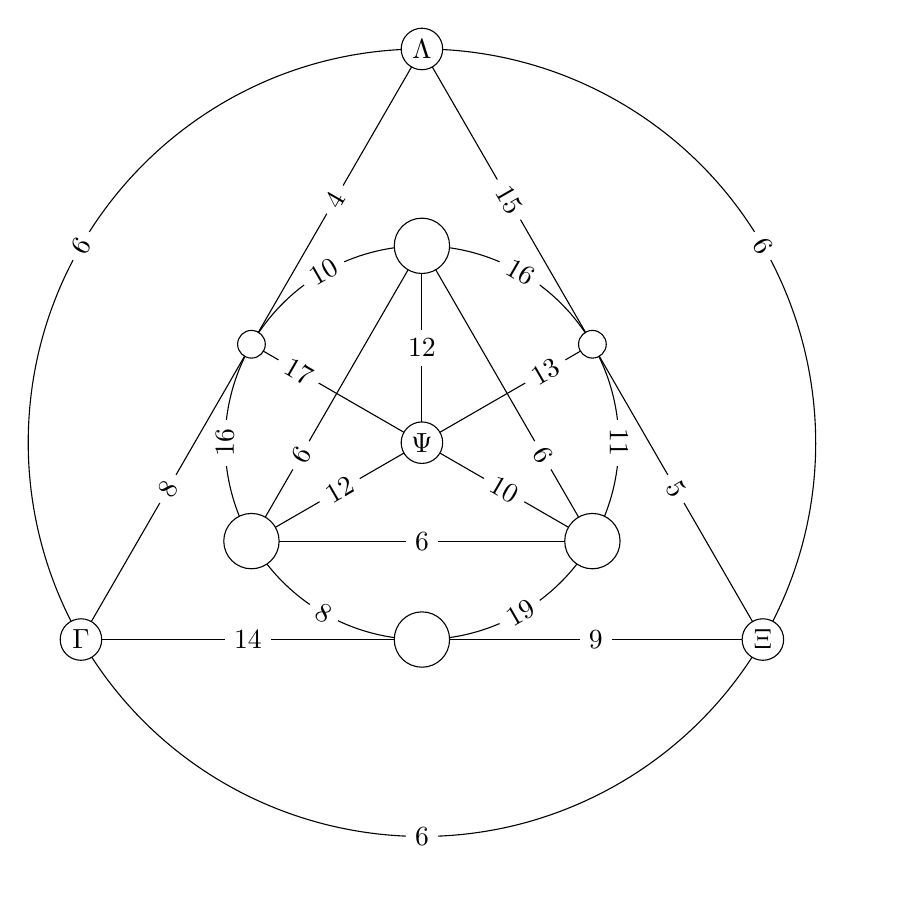
\begin{tikzpicture}
    [mynode/.style={draw,circle,inner sep = 0em, minimum size = 10}]

    % \node[draw, circle, minimum width=50mm, inner sep=0pt, outer sep=0pt] (inner) {};
    \graph[nodes={empty nodes}, clockwise, radius=50mm, n=3, name=outer] {subgraph I_n};
    \graph[nodes={empty nodes}, clockwise, radius=25mm, n=6, name=inner] {subgraph I_n};
    
    % \draw[-] (outer 1) -- (outer 2);
    % \draw[-] (outer 2) -- (outer 3);
    % \draw[-] (outer 3) -- (outer 1);
    
    \draw[-] (outer 1) arc[start angle=90, end angle=210, radius=50mm] node[midway, fill=white, sloped] {6};
    \draw[-] (outer 2) arc[start angle=-30, end angle=90, radius=50mm] node[midway, fill=white, sloped] {6};
    \draw[-] (outer 3) arc[start angle=210, end angle=330, radius=50mm] node[midway, fill=white, sloped] {6};
    
    \draw[-] (inner 1) arc[start angle=90, end angle=30, radius=25mm] node[midway, fill=white, sloped] {16};
    \draw[-] (inner 2) arc[start angle=30, end angle=-30, radius=25mm] node[midway, fill=white, sloped] {11};
    \draw[-] (inner 3) arc[start angle=330, end angle=270, radius=25mm] node[midway, fill=white, sloped] {19};
    \draw[-] (inner 4) arc[start angle=270, end angle=210, radius=25mm] node[midway, fill=white, sloped] {8};
    \draw[-] (inner 5) arc[start angle=210, end angle=150, radius=25mm] node[midway, fill=white, sloped] {16};
    \draw[-] (inner 6) arc[start angle=150, end angle=90, radius=25mm] node[midway, fill=white, sloped] {10};
    
    \node[draw, circle, minimum width=15, inner sep = 0pt, outer sep = 0pt, fill=white] (origo) at (0, 0) {$\Psi$};

    \node[draw, circle, minimum width=15, inner sep = 0pt, outer sep = 0pt, fill=white] (A) at (outer 1) {$\Lambda$};
    \node[draw, circle, minimum width=15, inner sep = 0pt, outer sep = 0pt, fill=white] (B) at (outer 2) {$\Xi$};
    \node[draw, circle, minimum width=15, inner sep = 0pt, outer sep = 0pt, fill=white] (C) at (outer 3) {$\Gamma$};

    \node[draw, circle, minimum width=20, inner sep = 0pt, outer sep = 0pt, fill=white] (1) at (inner 1) {};
    \node[draw, circle, minimum width=10, inner sep = 0pt, outer sep = 0pt, fill=white] (2) at (inner 2) {};
    \node[draw, circle, minimum width=20, inner sep = 0pt, outer sep = 0pt, fill=white] (3) at (inner 3) {};
    \node[draw, circle, minimum width=20, inner sep = 0pt, outer sep = 0pt, fill=white] (4) at (inner 4) {};
    \node[draw, circle, minimum width=20, inner sep = 0pt, outer sep = 0pt, fill=white] (5) at (inner 5) {};
    \node[draw, circle, minimum width=10, inner sep = 0pt, outer sep = 0pt, fill=white] (6) at (inner 6) {};
    
    \draw[-] (origo) -- (1) node[midway, fill=white] {12};
    \draw[-] (origo) -- (2) node[near end, fill=white, sloped] {13};
    \draw[-] (origo) -- (3) node[midway, fill=white, sloped] {10};
    \draw[-] (origo) -- (5) node[midway, fill=white, sloped] {12};
    \draw[-] (origo) -- (6) node[near end, fill=white, sloped] {17};
    \draw[-] (1) -- (3) node[near end, fill=white, sloped] {6};
    \draw[-] (3) -- (5) node[midway, fill=white, sloped] {6};
    \draw[-] (5) -- (1) node[near start, fill=white, sloped] {6};
    
    \draw[-] (A) -- (6) node[midway, fill=white, sloped] {4};
    \draw[-] (A) -- (2) node[midway, fill=white, sloped] {15};
    \draw[-] (B) -- (2) node[midway, fill=white, sloped] {5};
    \draw[-] (B) -- (4) node[midway, fill=white, sloped] {9};
    \draw[-] (C) -- (4) node[midway, fill=white, sloped] {14};
    \draw[-] (C) -- (6) node[midway, fill=white, sloped] {8};
    
\end{tikzpicture}
\end{document}